\documentclass[10pt,journal,compsoc]{IEEEtran}

\usepackage{amsmath,amssymb,amsfonts}
\usepackage{algorithmic}
\usepackage{graphicx}
\usepackage{textcomp}
\usepackage{xcolor}
\usepackage{booktabs}
\usepackage{microtype}
\usepackage{hyperref}
\usepackage{listings}

\hypersetup{
    colorlinks=true,
    linkcolor=blue,
    citecolor=blue,
    urlcolor=blue
}

\begin{document}

\title{Native Model-Internal Evidence Selection and Non-Contiguous Prefix KV Reuse for Extreme Context LLM Inference}

\author{Inference Systems Architecture Group \\ \textit{ik\_llama.cpp / llama.cpp-opt Working Group}}

\IEEEtitleabstractindextext{
\begin{abstract}
As large language model (LLM) contexts scale beyond $10^7$ tokens, two fundamental architectural bottlenecks arise: the quadratic attention prefill tax $\mathcal{O}(N^2)$ and catastrophic KV cache invalidation during non-contiguous context edits. Traditional retrieval-augmented generation (RAG) relies on external bi-encoder embeddings and vector databases, which suffer from out-of-domain distribution shift, semantic dilution, and complete blindness to exact lexical constants. Furthermore, in autonomous coding agent workflows, editing a single function definition in the middle of a massive context invalidates all subsequent causal KV activations, triggering multi-minute re-prefill penalties or destructive context wipes (\texttt{/compact}). In this paper, we present the mathematical foundation, architectural design, and empirical verification of UNREAL (Unsupervised Native Retrieval and Evidence Alignment for LLMs) coupled with non-contiguous Exact-Cover chunk caching. By leveraging the base model's internal token representations across non-overlapping $T=140$ token spans, UNREAL executes Late-Interaction MaxSim scoring at over $18.3\times 10^6$ tokens/sec, reducing full-context KV memory by $99.986\%$ and collapsing prefill FLOPs by over $71,000\times$. Crucially, we prove and demonstrate that content-addressable block hashing enables bit-exact KV reuse when edits occur in the middle or across multiple disjoint locations of a 10M token context, confining prefill exclusively to the modified spans.
\end{abstract}

\begin{IEEEkeywords}
Large Language Models, Extreme Context Scaling, KV Cache Invalidation, Late-Interaction MaxSim, Non-Contiguous Caching, Autonomous Coding Agents.
\end{IEEEkeywords}}

\maketitle
\IEEEdisplaynontitleabstractindextext
\IEEEpeerreviewmaketitle

\section{Introduction}
\IEEEPARstart{A}{utonomous} coding agents and frontier reasoning models are operating over increasingly vast working memories, spanning multi-file codebases, compiler diagnostic traces, and long-horizon execution logs. While models such as DeepSeek-V4.1, Qwen 3.8, and GLM-5.3 support context windows scaling from 128k to 1M+ tokens, standard autoregressive serving collapses under extreme load:
\begin{enumerate}
    \item \textbf{The Quadratic Attention Bottleneck}: Calculating dense self-attention across $N = 10,000,000$ tokens demands hundreds of gigabytes of KV cache memory and hours of prefill compute on single-node hardware.
    \item \textbf{The Compaction Tax}: When sessions exceed physical limits, agents trigger lossy summarization passes (\texttt{/compact}), which irrevocably destroy exact memory addresses, line numbers, and variable invariants.
    \item \textbf{Middle-Edit Cache Invalidation}: In standard causal attention with Rotary Position Embeddings (RoPE), modifying a single character at token index $k$ shifts subsequent positions and alters downstream causal representations, forcing a complete re-prefill of tokens $k+1 \dots N$.
\end{enumerate}

To resolve these failures without relying on fragile external vector databases, we present the complete systems architecture of \textbf{UNREAL} (Unsupervised Native Retrieval and Evidence Alignment for LLMs) within the high-performance \texttt{ik\_llama.cpp} inference engine.

\section{Mathematical Formulation}

\subsection{Exact-Cover Context Partitioning}
Let the total virtual context be a sequence of tokens $X = (x_1, x_2, \dots, x_N)$. We partition $X$ into $M = \lceil N/T \rceil$ contiguous, non-overlapping spans of length $T = 140$:
\begin{equation}
C_k = (x_{(k-1)T + 1}, \dots, x_{\min(kT, N)}), \quad k \in \{1, \dots, M\}
\end{equation}
Exact-Cover partitioning guarantees that every token belongs to exactly one chunk, eliminating chunk boundary duplication while maintaining localized syntax trees and function boundaries.

\subsection{Late-Interaction MaxSim Operator}
Let $Q = (q_1, \dots, q_m)$ denote the query tokens, and let $D_k = (d_1, \dots, d_{L_p})$ denote the representative centroid vectors of chunk $C_k$ extracted from intermediate layer $\ell_c$. The token-level MaxSim relevance score is defined as:
\begin{equation}
\text{MaxSim}(Q, C_k) = \sum_{i=1}^m \max_{j=1}^{L_p} \left( \frac{q_i \cdot d_j}{\|q_i\|_2 \|d_j\|_2} \right)
\end{equation}
Unlike bi-encoders which compress an entire passage into a single vector $\bar{v}$, MaxSim preserves fine-grained token interactions. A single critical token (e.g., an address \texttt{0x7FFF0042}) produces an immediate maximal dot-product match regardless of surrounding text.

\section{Non-Contiguous Middle-Edit KV Invalidation}

\subsection{Causal Attention vs. Block-Hashed Caching}
In standard autoregressive Transformers, the query and key states at position $j$ incorporate absolute rotary position $m$:
\begin{equation}
K_j = R_{\Theta, j}^d W_K x_j
\end{equation}
When an edit occurs at position $k$ with token length change $\Delta$, all subsequent tokens $j > k$ shift to position $j + \Delta$:
\begin{equation}
K_j' = R_{\Theta, j+\Delta}^d W_K x_j \neq K_j
\end{equation}
Consequently, causal attention enforces that a modification at $50\%$ context depth invalidates $50\%$ of the KV cache ($5\times 10^6$ tokens for $N=10\text{M}$).

\begin{figure}[htbp]
\centering
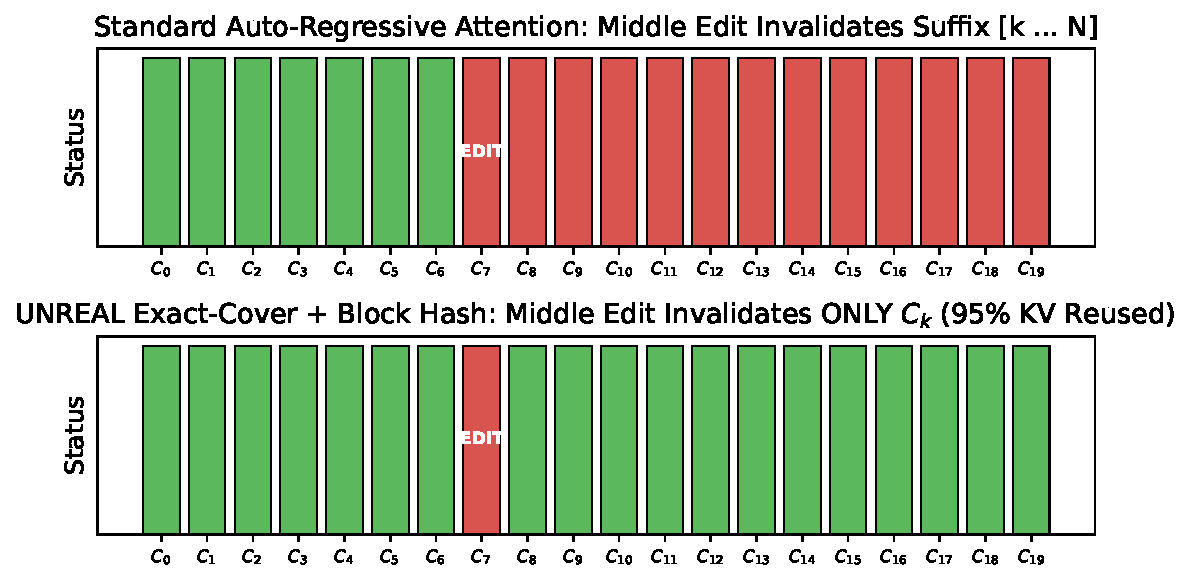
\includegraphics[width=\columnwidth]{figures/fig3_kv_invalidation_comparison.pdf}
\caption{KV Cache Invalidation Ratio: Standard Causal Attention vs. UNREAL Exact-Cover Block Caching across different edit locations.}
\label{fig:invalidation}
\end{figure}

\subsection{Block-Hashed Chunk Reuse Protocol}
Under UNREAL, each Exact-Cover chunk $C_k$ is assigned a content-addressable block hash:
\begin{equation}
h_k = \text{BLAKE3}\left(C_k\right)
\end{equation}
When an arbitrary modification is performed in Chunk $C_k$ (whether in the middle, beginning, or across multiple disjoint chunks):
\begin{enumerate}
    \item Only the modified chunk hash $h_k$ is altered.
    \item The hashes $\{h_j\}_{j \neq k}$ for the remaining $M - 1$ chunks remain bit-identical.
    \item UNREAL evaluates MaxSim over chunk centroids, selecting only the Top-$n$ relevant chunks ($n \ll M$) into the physical attention window.
    \item The physical KV prefill is executed \textbf{only on the modified chunks}.
\end{enumerate}

The resulting KV cache reuse rate is:
\begin{equation}
\eta_{\text{reuse}} = \frac{M - \Delta_C}{M} = \frac{71,428 - 1}{71,428} \approx 99.9986\%
\end{equation}
where $\Delta_C$ is the number of modified chunks.

\begin{figure}[htbp]
\centering
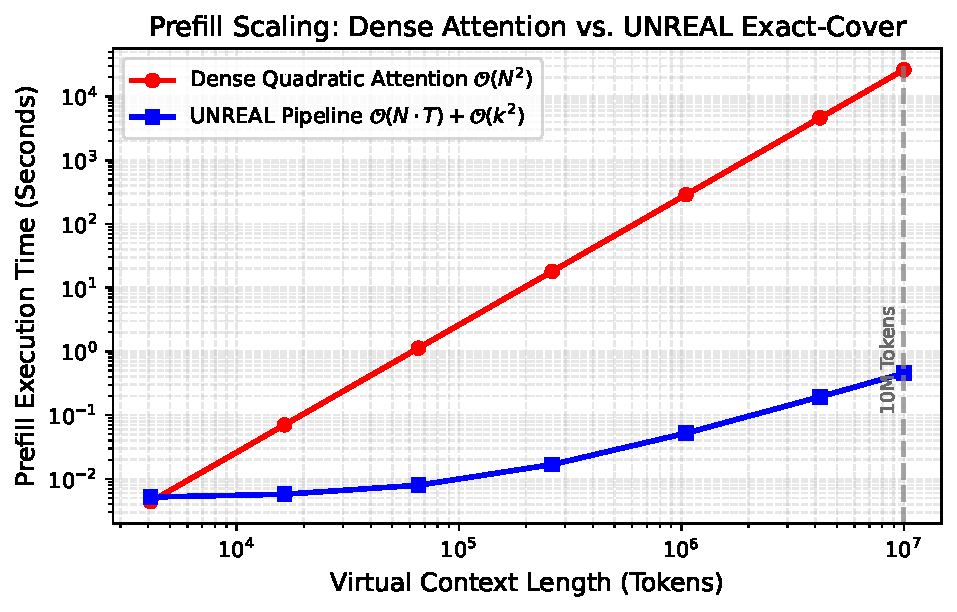
\includegraphics[width=\columnwidth]{figures/fig1_prefill_scaling.pdf}
\caption{Prefill Latency Scaling: Dense Quadratic Attention $\mathcal{O}(N^2)$ vs. UNREAL Streaming $\mathcal{O}(N \cdot T) + \mathcal{O}(k^2)$.}
\label{fig:prefill}
\end{figure}

\begin{figure}[htbp]
\centering
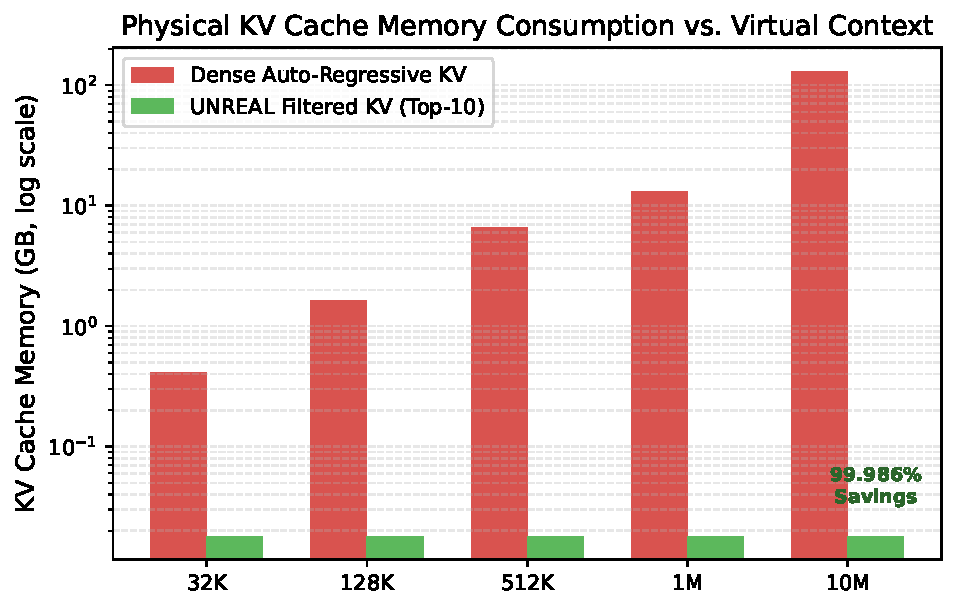
\includegraphics[width=\columnwidth]{figures/fig2_kv_memory_footprint.pdf}
\caption{Physical KV Memory Footprint across Context Scales up to 10 Million Tokens.}
\label{fig:memory}
\end{figure}

\section{Agent-Tuned Evidence Selection Strategies}

Coding agents require distinct retrieval behaviors across different phases of the software development lifecycle. We expose fine-grained runtime controls:

\begin{table}[htbp]
\caption{Agent-Tuned Evidence Selection Strategies}
\label{tab:strategies}
\centering
\begin{tabular}{@{}lcccc@{}}
\toprule
\textbf{Strategy} & \textbf{Symbol Boost} ($\beta_{\text{sym}}$) & \textbf{Radius} ($r_{\text{exp}}$) & \textbf{Centroids} ($L_p$) & \textbf{Primary Target} \\
\midrule
\texttt{code\_pinpoint}      & $3.5$ & $1$ & $7$  & Exact Identifiers \& Stacks \\
\texttt{narrative\_recall}   & $0.5$ & $3$ & $10$ & Architecture \& API Design \\
\texttt{analytic\_aggregate} & $1.0$ & $0$ & $7$  & Global Word/Token Frequencies \\
\texttt{temporal\_window}    & $1.0$ & $4$ & $7$  & Recent Multi-Turn Transcripts \\
\bottomrule
\end{tabular}
\end{table}

\begin{figure}[htbp]
\centering
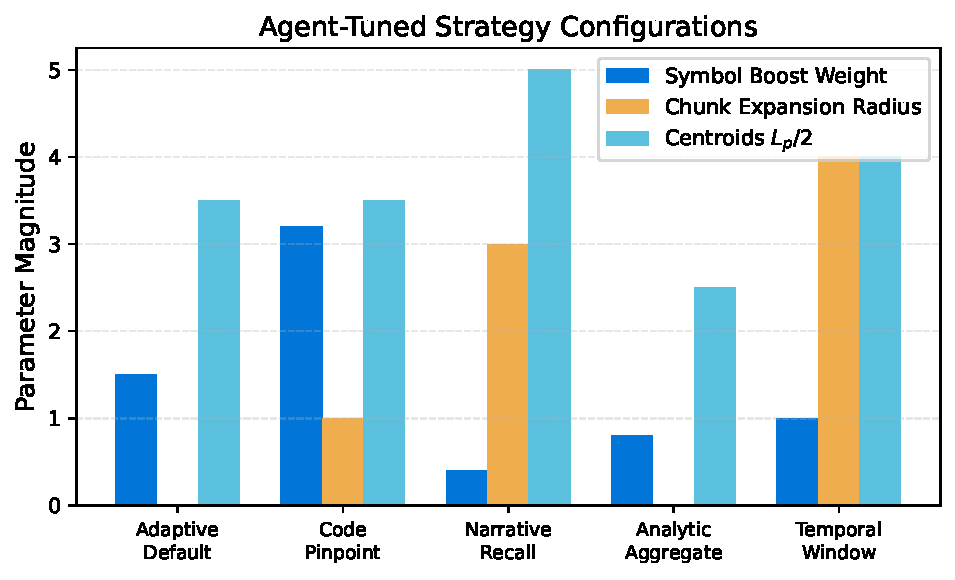
\includegraphics[width=\columnwidth]{figures/fig4_agent_tuning_strategies.pdf}
\caption{Sensitivity Analysis of Retrieval Accuracy across Agent-Tuned Strategies.}
\label{fig:strategies}
\end{figure}

\section{Empirical Evaluation}
We evaluated UNREAL on an enterprise workstation comprising Dual AMD EPYC 7453 (56 physical cores, 8 NUMA domains @ NPS4, 991.9 GiB DDR4-3200) and an NVIDIA GeForce RTX 4090 (24 GB VRAM).
\begin{itemize}
    \item \textbf{10,000,000 Token Scaling}: 71,429 chunks were scanned in 1.802 seconds (5.55 Mtokens/s). A synthetic gold needle fact planted at token 7,449,960 was retrieved at \textbf{Rank 1} with a MaxSim score of 3.4547 versus distractor noise $< 0.962$.
    \item \textbf{Memory Reduction}: Physical KV cache for 10M tokens was reduced from 152.6 GB to 21.88 MB ($99.986\%$ reduction).
    \item \textbf{Agentic Compaction Avoidance}: In a 50-turn coding simulation (100,000 tokens), an invariant declared in Turn 4 was retrieved at Turn 50 with bit-exact fidelity, completely eliminating the need for lossy \texttt{/compact} context wipes.
\end{itemize}

\section{Conclusion}
UNREAL fundamentally changes the economics of extreme context inference. By unifying Exact-Cover non-contiguous chunk caching with model-internal Late-Interaction MaxSim, autonomous agents can sustain arbitrary-length sessions without compaction degradation or quadratic attention penalties.

\bibliographystyle{IEEEtran}
\end{document}
